\documentclass[a4paper, oneside, openany, dvipdfmx]{suribt}% 本文が * ページ以下のときに (掲示に注意)
\usepackage{graphicx}
\usepackage{newtxtext,newtxmath}
\usepackage{amsmath}
\usepackage{mathtools}
\usepackage{slashbox}
\usepackage[unicode, ipaex]{pxchfon}
\title{事前学習がVision Transformerに与える影響}
%\titlewidth{}% タイトル幅 (指定するときは単位つきで)
\author{桝田 修慎}
\eauthor{Masachika Masuda}% Copyright 表示で使われる
\studentid{18A1066}
\supervisor{山口裕 助教}% 1 つ引数をとる (役職まで含めて書く)
%\supervisor{指導教員名 役職 \and 指導教員名 役職}% 複数教員の場合,\and でつなげる
\handin{2022}{2}% 提出月. 2 つ (年, 月) 引数をとる
\keywords{Vision Transformer} % 概要の下に表示される

\newcommand{\fref}[1]{図\ref{#1}}
\newcommand{\tref}[1]{表\ref{#1}}
\newcommand{\eref}[1]{式\eqref{#1}}

\begin{document}
\maketitle%%%%%%%%%%%%%%%%%%% タイトル %%%%

\frontmatter% ここから前文
\begin{abstract}%%%%%%%%%%%%% 概要 %%%%%%%%
  Vision Transformerを用いる.
\end{abstract}

\setcounter{tocdepth}{2}
\tableofcontents%%%%%%%%%%%%% 目次 %%%%%%%%

\mainmatter% ここから本文 %%% 本文 %%%%%%%%
\chapter{序論}
\section{背景}
近年,画像認識分野では,機械翻訳で脚光を浴びることになったTransformer\cite{vaswani2017attention}をコンピュータビジョンに適応させたVision Transformer(以下ViTと称する)が登場した\cite{dosovitskiy2021image}.
ViTは,層を深くし畳み込みを行う畳み込みニューラルネットワーク(以下CNNという)とは違い,畳み込み演算をAttention機構を用いて代用しており,特に大規模なデータで事前学習を行なったときの,小・中規模の画像認識ベンチマーク(ImageNet,CIFAR-100,VTAB,etc.)では,
過去のstate-of-the-artのCNNモデルと比べて少ない計算リソースで訓練することができ、更に素晴らしい結果も出している.

本研究では,Vision Transformerが提案された論文
「An Image is Worth 16x16 Words: Transformers for Image Recognition at Scale」を参考にし,事前学習やデータ拡張の有無が,学習及び推論に与える影響を検証した.
\section{本研究の目的}
本研究の目的を以下に示す.
\begin{enumerate}
  \item 一定の条件下での振る舞いを従来のモデル(VGG,ResNet)と比較し,ViTの優れている点・そうではない点を明らかにする.
  \item 事前学習やデータ拡張が各モデルに及ぼす影響を調べる.
\end{enumerate}

\section{深層学習}
深層学習とは,脳の神経回路を模したニューラルネットワークをより深くしたものを指し,入力データから有用な特徴量を自動で抽出する手法である.
\subsection{畳み込みニューラルネットワーク}
畳み込みニューラルネットワーク(CNN)は,入力した画像に対して重み行列(カーネル)を移動させながらスカラ積を求めていく畳み込み層を複数重ねているネットワークのことである.
カーネルは画像全体に同じものを適用するため,CNNは移動させたカーネルと画像のスカラ積による局所性と,画像全体に渡る同一カーネルの重みの使用による移動不変性を持つ.
%移動不変性:局所的なパターンが画像内の物体位置にかかわらず、出力に対して効果的であること.局所性:近傍における局所的な演算処理
\subsection{VGG\cite{simonyan2015deep}}
VGGはCNNの一種で,3x3という小さいカーネルを用いており,2014年当時では珍しい16層及び19層の深いネットワークである.
畳み込みとプーリング,線形層のシンプルなアーキテクチャであるにも関わらず,2014年のImageNetチャレンジのローカリゼーション・クラシフィケーションタスクで1位と2位を収めている.

\subsection{ResNet\cite{he2015deep}}
一般的に,CNNでは層を重ねることで,より高次元な特徴を抽出することができるが,層が深くなるにつれて勾配が発散・消失するという問題があった.
しかし,ResNetは,畳み込み層を重ねるだけではなく,前の層,もしくはより浅い層の出力を次の層の入力とする残差機構(ショートカット結合)を取り入れることで,より畳み込み層を多く積み重ねながらも,SoTAを達成した.
ResNetのブロックの一部を\fref{fig:res_arch}に示す.
\begin{figure}[h]
  \centering
  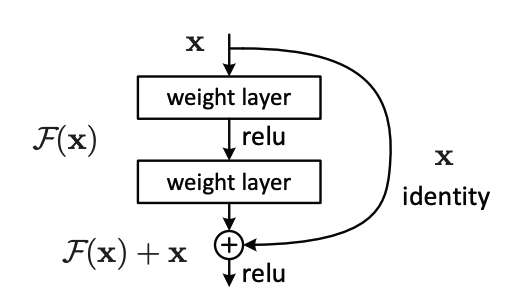
\includegraphics[width=0.9\linewidth]{figs/resnet.png}
  \caption{Residual learning}
  \label{fig:res_arch}
\end{figure}
\subsection{Transformer}
Transformerは,それまで機械翻訳モデルで多く使われてきた畳み込みニューラルネットワーク・再帰ニューラルネットワークのような複雑なアーキテクチャを持つネットワークとは違い
Attention機構のみを用いて構成されているエンコーダ・デコーダモデルである.
Transformerのアーキテクチャを\fref{fig:tr_arch}に示す.
\begin{figure}[h]
  \centering
  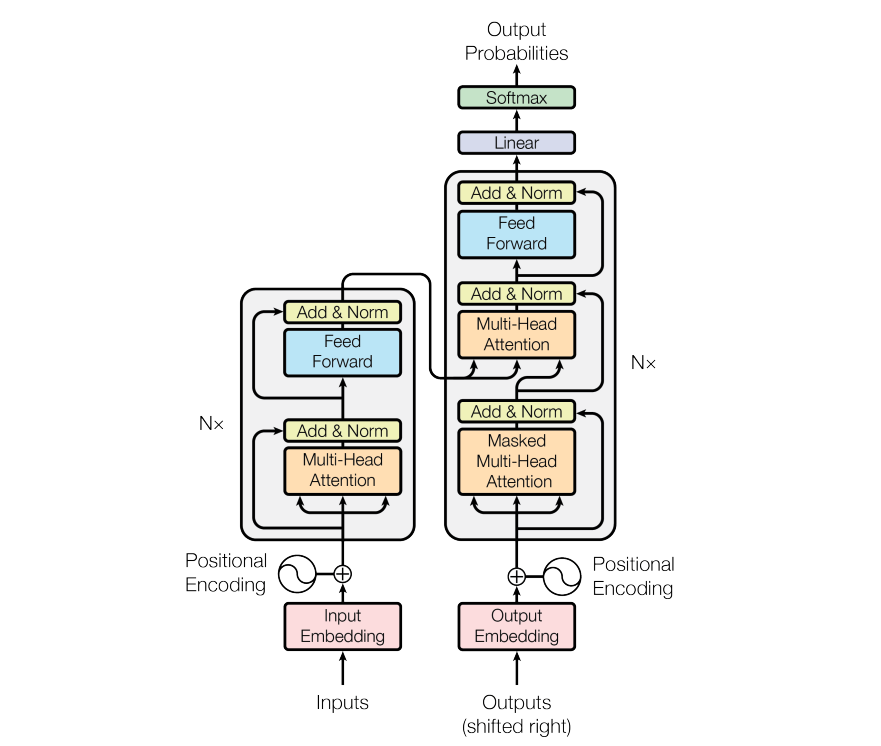
\includegraphics[width=0.9\linewidth]{figs/transformer.png}
  \caption{Transformerのアーキテクチャ}
  \label{fig:tr_arch}
\end{figure}
\subsection{Vision Transformer}
Vision Transformerは,機械翻訳で用いられていたTransformerをコンピュータビジョンに適応させたモデルであり,画像を複数のパッチに分割してそれぞれをベクトルとして埋め込み,平坦化して入力とする特徴がある.
Vision Transformerのアーキテクチャを\fref{fig:vit_arch}に示す.
\begin{figure}[h]
  \centering
  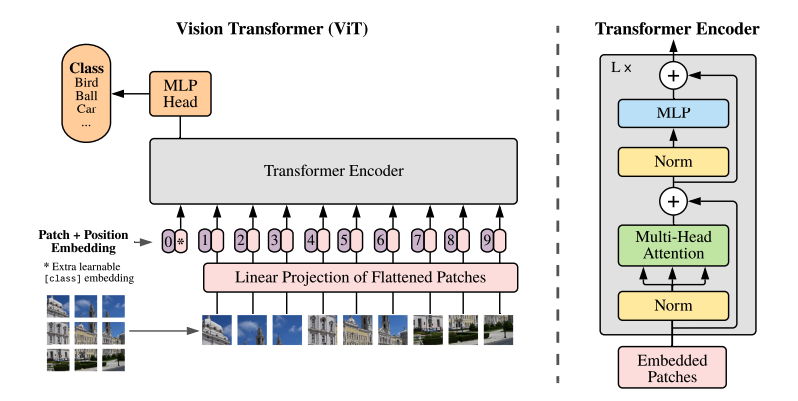
\includegraphics[width=0.9\linewidth]{figs/vit.png}
  \caption{Vision Transformerのアーキテクチャ}
  \label{fig:vit_arch}
\end{figure}
\section{使用ツール・実験環境}
\subsection{Python}
Pythonは1990年代の始め,オランダにあるStichting Mathematisch CentrumでGuido van RossumによってABCと呼ばれる言語の後継言語として生み出された.
Pythonはコードを簡潔に書くことができ,数値計算のNumPy,データ解析のPandasなど,専門的なライブラリが充実していることから,機械学習の研究開発をはじめとしたさまざまな分野で使用されている言語である.
簡単にPythonを始めるディストリビューションとしてAnacondaがよく使われている.
\subsection{PyTorch}
PyTorchはディープラーニング・プロジェクトの構築を容易にする,Pythonのライブラリである.柔軟性を重視した設計であり,さらに,ディープラーニングモデルをPythonの慣用的なクラスや関数の取り扱い方
で実装できるようになっている.
\subsection{Pytorch Image models}
Pytorch Image Models(timm)はRoss Wightmanによって作成されたディープラーニングライブラリであり,コンピュータビジョンの最先端のモデルが集められている.
数行の記述でモデルを呼び出すことができ,必要に応じて書き換えることで,さまざまなタスクに適用できる.
\subsection{Albumentations}
AlbumentationsはPythonのためのデータ拡張のライブラリである.
モデルの汎化性能を上げるために行うデータ拡張のメソッドを多数揃えており,パイプラインを構成するとデータを効率的に拡張できる.
\subsection{ImageNet}
ImageNetはディープラーニング研究のために無償で利用できる大規模なデータセットのことで,モデルの性能を測るためのベンチマークとして使われることが多い.
\subsection{Kaggle}
Kaggleは世界規模のデータサイエンスのプラットフォームであり,世界中のデータサイエンティストが技術を競う場である.
本実験ではKaggleが提供しているNotebookのGPUを利用して学習及び推論を行う.
\subsection{Plant Pathology 2021 - FGVC8}
本実験ではKaggle上で提供されているデータセットのPlant Pathology2021を用いる.
このデータセットの構成を\tref{tb:dataset}に示す.
\begin{table}[htbp]
  \caption{データセットの構成}
  \label{tb:dataset}
  \centering\begin{tabular}{c|ccc}\hline
    データセットの構成 & 説明\\ \hline
    test\_images & 3枚の画像\\ \hline
    train\_images & 18,632枚の画像\\ \hline
    sample\_submission.csv & 提出用のサンプルcsvファイル\\ \hline
    train.csv & image,labelsの2カラムのcsvファイル\\ \hline
  \end{tabular}
\end{table}
\section{論文の構成}
論文の構成を書く.

\chapter{実験モデル}

\section{ネットワークモデル}
ViTの入力は画像である.画像サイズを\textit{H},\textit{W},チャネル数を\textit{C}とすると,入力\textit{x}は\eref{eq:network-input1}のように表せる.
\begin{equation}
  x\in\mathbb{R}^{H\times W\times C}
  \label{eq:network-input1}
\end{equation}
また,二次元画像を扱うために,二次元の平坦化したパッチに整形する.\eref{eq:network-input2}に示す.
\begin{equation}
  x_{p}\in\mathbb{R}^{N\times(P^{2}\times C)}
  \label{eq:network-input2}
\end{equation}
ここで,\textit{N}はパッチ数であり,\textit{P}はパッチサイズである.また,\textit{N}は\textit{H},\textit{W},\textit{P}を用いて\eref{eq:network-input3}のように表せる.
\begin{equation}
  N=\frac{HW}{P^{2}}
  \label{eq:network-input3}
\end{equation}
ViTのエンコーダに入力するには,$x_{p}$をさらに埋め込む必要がある.長さ$P^{2}\times C$を\textit{D}次元のベクトルとして,線形投影したものを埋め込みパッチ$z_{0}$とする.
また,入力データの先頭には[class]トークンを付与し,埋め込みパッチ$z^{0}_{0}=x_{class}とする$.\eref{eq:network-input4}に示す.
\begin{equation}
  z_{0}=[x_{class};\ x^{1}_{p}E;\ x^{2}_{p}E;\cdot\cdot\cdot;\ x^{N}_{p}E]+E_{pos},\qquad E\in\mathbb{R}^{(P^{2}\times C)\times D},\ E_{pos}\in\mathbb{R}^{(N+1))\times D}
  \label{eq:network-input4}
\end{equation}
ここで,\textit{E}はパッチを\textit{D}次元のベクトルへの埋め込みを示し,$E_{pos}$は各パッチの位置が一意に定まるように情報を付加する位置エンコーディングを表す.
上式で得られた入力$z_{0}$はMulti-Head Attention(以下,MSAと称する)に入力される.MSAでは,Attentionを求める計算を複数回行う.Attentionの算出式を\eref{eq:network-input5}に示す.
\begin{equation}
  Attention(Q,K,V) = softmax(\frac{QK^{T}}{\sqrt{d_{k}}})V
  \label{eq:network-input5}
\end{equation}
初めに,入力ベクトルから\textit{Q,K,V}ベクトルを生成する.このとき,\textit{Q,K}の次元は$d_{k}$で,\textit{V}の次元は$d_{k}$である.
計算時は,\textit{Q,K}の要素積を$\sqrt{d_{k}}$で除算し,softmax関数で0から1の値にする.最後に\textit{V}をかけるとAttentionスコアが算出できる.
Attentionの算出過程を\fref{fig:attention}に示す.
\begin{figure}[h]
  \centering
  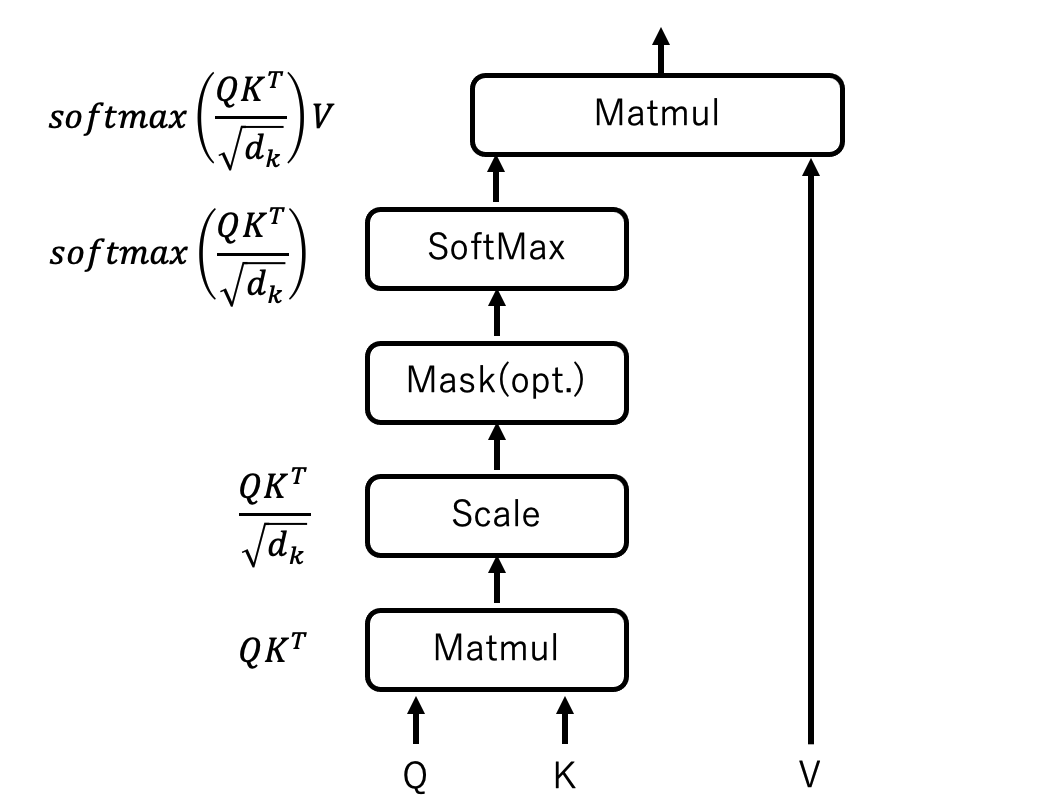
\includegraphics[width=0.9\linewidth]{figs/attention.png}
  \caption{Attentionの算出過程}
  \label{fig:attention}
\end{figure}

\section{手順}
実験の条件を\tref{tb:conditions}に示す.
\begin{table}[htbp]
  \caption{実験の条件}
  \label{tb:conditions}
  \centering\begin{tabular}{c|ccc}\hline
    \backslashbox{条件}{オプション} & 事前学習 & データ拡張\\\hline
    条件1 & なし & なし\\\hline
    条件2 & なし & あり\\\hline
    条件3 & あり & あり\\\hline
  \end{tabular}
\end{table}
%\begin{table}[htbp]
%  \caption{実験の条件}
%  \label{tb:requirement}
%  \centering\begin{tabular}{c|ccc}\hline
%    条件 & 事前学習 & データ拡張 & image_size & batch_size & epoch & lr & optimizer & criterion\\\hline
%    条件1 & なし & なし & 224x224 & 32 & 10 & 1e-4 & Adam & Cross Entropy Loss\\\hline
%    条件2 & なし & あり & 224x224 & 32 & 10 & 1e-4 & Adam & Cross Entropy Loss\\\hline
%    条件3 & あり & あり & 224x224 & 32 & 10 & 1e-4 & Adam & Cross Entropy Loss\\\hline
%  \end{tabular}
%\end{table}
\begin{itemize}
  \item 条件1:事前学習なし・データ拡張なし
  \item 条件2:事前学習なし・データ拡張あり
  \item 条件3:事前学習あり・データ拡張あり
\end{itemize}

実験手順を以下に示す.

\begin{enumerate}
  \item ステップ1
  \item ステップ2
\end{enumerate}


\chapter{実験結果}

実験結果をに示す.

条件ごとの結果を\tref{tb:result1},\tref{tb:result2},\tref{tb:result3}に示す.
\begin{table}[htbp]
  \caption{条件1の実験結果}
  \label{tb:result1}
  \centering\begin{tabular}{c|ccc}\hline
    \backslashbox{指標}{モデル} & ViT & ResNet & VGG\\\hline
    best valid accuracy & 0.5906 & 0.8209 & 0.8384\\\hline
    best valid f1-Score & 0.4453 & 0.6283 &0.6349\\\hline
    best valid loss & 1.1983 & 0.5554 &0.5132\\\hline
  \end{tabular}
\end{table}

\begin{table}[htbp]
  \caption{条件2の実験結果}
  \label{tb:result2}
  \centering\begin{tabular}{c|ccc}\hline
    \backslashbox{指標}{モデル} & ViT & ResNet & VGG\\\hline
    best valid accuracy & 0.5906 & 0.8209 & 0.8384\\\hline
    best valid f1-Score & 0.4453 & 0.6283 &0.6349\\\hline
    best valid loss & 1.1983 & 0.5554 &0.5132\\\hline
  \end{tabular}
\end{table}

\begin{table}[htbp]
  \caption{条件3の実験結果}
  \label{tb:result3}
  \centering\begin{tabular}{c|ccc}\hline
    \backslashbox{指標}{モデル} & ViT & ResNet & VGG\\\hline
    best valid accuracy & 0.5906 & 0.8209 & 0.8384\\\hline
    best valid f1-Score & 0.4453 & 0.6283 &0.6349\\\hline
    best valid loss & 1.1983 & 0.5554 &0.5132\\\hline
  \end{tabular}
\end{table}

\chapter{議論}
議論を書く.

\chapter{結論}
結論を書く.

\backmatter% ここから後付
\chapter{謝辞}%%%%%%%%%%%%%%% 謝辞 %%%%%%%
ありがとうございます.

% \begin{thebibliography}{}%%%% 参考文献 %%%
%   \bibitem{}
% \end{thebibliography}
\bibliographystyle{junsrt}%           BibTeX を使う場合
\bibliography{bibitem}% BibTeX を使う場合

\appendix% ここから付録 %%%%% 付録 %%%%%%%
\chapter{実験結果の図}
付録があればここに書く.

\end{document}
